% questions.tex —— 2006 年·四川卷·文科 · 题目内容片段（无答案）
% 由 tools/generate_projects.py 依来源总账自 2006/2006_数学真题_四川文_试题.md 生成，勿手改（改源 MD 后重跑）


\begin{gktip}
\textbf{来源边界}：题签依据固定 PDF 首页照录。题面按固定 PDF 第1—2页转录，印刷页码为334—335。固定副本的发布者、出版者、版次、来源链及官方身份均未核；\texttt{ready} 仅为来源清单中的文件状态，不代表来源认证。固定 PDF 可见范围未见答案、解析、评分或总分。
\end{gktip}

\gkpart{一、选择题}

\begin{question}
\gkti{1}已知集合 $A=\{x\mid x^2-5x+6\leqslant0\}$，集合 $B=\{x\mid |2x-1|>3\}$，则集合 $A\cap B=$\mbox{（　　）}。

（A）$\{x\mid 2\leqslant x\leqslant3\}$　　（B）$\{x\mid 2\leqslant x<3\}$

（C）$\{x\mid 2<x\leqslant3\}$　　（D）$\{x\mid -1<x<3\}$

\end{question}
\begin{question}
\gkti{2}函数 $f(x)=\ln(x-1)\ (x>1)$ 的反函数是\mbox{（　　）}。

（A）$f^{-1}(x)=e^x+1\ (x\in\mathbb R)$　　（B）$f^{-1}(x)=10^x+1\ (x\in\mathbb R)$

（C）$f^{-1}(x)=10^x+1\ (x>1)$　　（D）$f^{-1}(x)=e^x+1\ (x>1)$

\end{question}
\begin{question}
\gkti{3}曲线 $y=4x-x^3$ 在点 $(-1,-3)$ 处的切线方程是\mbox{（　　）}。

（A）$y=7x+4$　　（B）$y=7x+2$　　（C）$y=x-4$　　（D）$y=x-2$

\Needspace{0.4\textheight}
\end{question}
\begin{question}
\gkti{4}如图，已知正六边形 $P_1P_2P_3P_4P_5P_6$，下列向量的数量积中最大的是\mbox{（　　）}。
\nopagebreak[4]
\begin{center}% Q4: regular hexagon from the fixed candidate PDF, printed page 334.
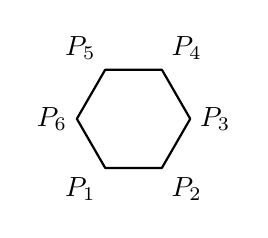
\begin{tikzpicture}[line cap=round,line join=round,x=0.72cm,y=0.72cm]
  \coordinate (P1) at (0,0);
  \coordinate (P2) at (1,0);
  \coordinate (P3) at (1.5,0.866);
  \coordinate (P4) at (1,1.732);
  \coordinate (P5) at (0,1.732);
  \coordinate (P6) at (-0.5,0.866);
  \draw[thick] (P1)--(P2)--(P3)--(P4)--(P5)--(P6)--cycle;
  \node[below left] at (P1) {$P_1$};
  \node[below right] at (P2) {$P_2$};
  \node[right] at (P3) {$P_3$};
  \node[above right] at (P4) {$P_4$};
  \node[above left] at (P5) {$P_5$};
  \node[left] at (P6) {$P_6$};
\end{tikzpicture}
\end{center}
\nopagebreak[4]
（A）$\overrightarrow{P_1P_2}\cdot\overrightarrow{P_1P_3}$　　（B）$\overrightarrow{P_1P_2}\cdot\overrightarrow{P_1P_4}$

（C）$\overrightarrow{P_1P_2}\cdot\overrightarrow{P_1P_5}$　　（D）$\overrightarrow{P_1P_2}\cdot\overrightarrow{P_1P_6}$

\end{question}
\begin{question}
\gkti{5}甲校有3600名学生，乙校有5400名学生，丙校有1800名学生，为统计三校学生某方面的情况，计划采用分层抽样法，抽取一个容量为90人的样本，应在这三校分别抽取学生\mbox{（　　）}。

（A）30人，30人，30人　　（B）30人，45人，15人

（C）20人，30人，10人　　（D）30人，50人，10人

\Needspace{0.4\textheight}
\end{question}
\begin{question}
\gkti{6}下列函数中，图象的一部分如图所示的是\mbox{（　　）}。
\nopagebreak[4]
\begin{center}% Q6: schematic cosine graph with the source's labelled intercept and maximum.
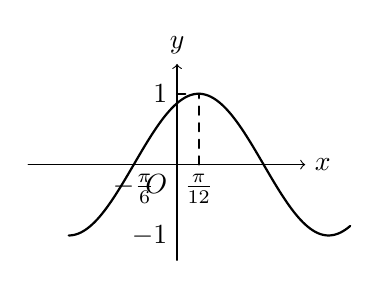
\begin{tikzpicture}[line cap=round,line join=round,x=1.05cm,y=0.9cm]
  \draw[->] (-1.8,0)--(1.55,0) node[right] {$x$};
  \draw[->] (0,-1.35)--(0,1.42) node[above] {$y$};
  \draw[thick,dashed] ({pi/12},0)--({pi/12},1);
  \draw[thick,dashed] (0,1)--({pi/12},1);
  \draw[thick,domain=-75:120,samples=120,variable=\t]
    plot ({\t*pi/180},{cos(2*\t-30)});
  \node[below left] at (0,0) {$O$};
  \node[left] at (0,1) {$1$};
  \node[left] at (0,-1) {$-1$};
  \node[below] at ({-pi/6},0) {$-\frac{\pi}{6}$};
  \node[below] at ({pi/12},0) {$\frac{\pi}{12}$};
\end{tikzpicture}
\end{center}
\nopagebreak[4]
（A）$y=\sin\left(x+\dfrac\pi6\right)$　　（B）$y=\sin\left(2x-\dfrac\pi6\right)$

（C）$y=\cos\left(4x-\dfrac\pi3\right)$　　（D）$y=\cos\left(2x-\dfrac\pi6\right)$

\end{question}
\begin{question}
\gkti{7}已知二面角 $\alpha-l-\beta$ 的大小为 $60^\circ$，$m,n$ 为异面直线，且 $m\perp\alpha$，$n\perp\beta$，则 $m,n$ 所成的角为\mbox{（　　）}。

（A）$30^\circ$　　（B）$60^\circ$　　（C）$90^\circ$　　（D）$120^\circ$

\end{question}
\begin{question}
\gkti{8}已知两定点 $A(-2,0)$、$B(1,0)$，如果动点 $P$ 满足 $|PA|=2|PB|$，则点 $P$ 的轨迹所围图形的面积等于\mbox{（　　）}。

（A）$9\pi$　　（B）$8\pi$　　（C）$4\pi$　　（D）$\pi$

\Needspace{0.4\textheight}
\end{question}
\begin{question}
\gkti{9}如图，正四棱锥 $P-ABCD$ 底面的四个顶点 $A\text{、}B\text{、}C\text{、}D$ 在球 $O$ 的同一个大圆上，点 $P$ 在球面上，如果 $V_{P-ABCD}=\dfrac{16}{3}$，则球 $O$ 的表面积是\mbox{（　　）}。
\nopagebreak[4]
\begin{center}% Q9: sphere containing a regular square pyramid whose base lies in a great circle.
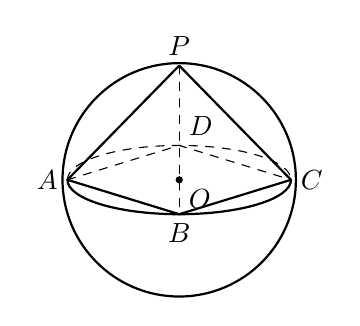
\begin{tikzpicture}[line cap=round,line join=round,x=0.78cm,y=0.78cm]
  \coordinate (O) at (0,0);
  \coordinate (P) at (0,1.86);
  \coordinate (A) at (-1.82,0);
  \coordinate (B) at (0,-0.56);
  \coordinate (C) at (1.82,0);
  \coordinate (D) at (0,0.56);
  \draw[thick] (O) circle (1.9);
  \draw[dashed] (A) arc[start angle=180,end angle=0,x radius=1.82,y radius=0.56];
  \draw[thick] (A) arc[start angle=180,end angle=360,x radius=1.82,y radius=0.56];
  \draw[thick] (A)--(B)--(C);
  \draw[dashed] (A)--(D)--(C);
  \draw[thick] (P)--(A) (P)--(C);
  \draw[dashed] (P)--(B) (P)--(D);
  \fill (O) circle (1.3pt);
  \node[above] at (P) {$P$};
  \node[left] at (A) {$A$};
  \node[below] at (B) {$B$};
  \node[right] at (C) {$C$};
  \node[above right] at (D) {$D$};
  \node[below right] at (O) {$O$};
\end{tikzpicture}
\end{center}
\nopagebreak[4]
（A）$4\pi$　　（B）$8\pi$　　（C）$12\pi$　　（D）$16\pi$

\end{question}
\begin{question}
\gkti{10}直线 $y=x-3$ 与抛物线 $y^2=4x$ 交于 $A\text{、}B$ 两点，过 $A\text{、}B$ 两点向抛物线的准线作垂线，垂足分别为 $P\text{、}Q$，则梯形 $APQB$ 的面积为\mbox{（　　）}。

（A）36　　（B）48　　（C）56　　（D）64

\end{question}
\begin{question}
\gkti{11}设 $a\text{、}b\text{、}c$ 分别是 $\triangle ABC$ 的三个内角 $A\text{、}B\text{、}C$ 所对的边，则 $a^2=b(b+c)$ 是 $A=2B$ 的\mbox{（　　）}。

（A）充要条件　　（B）充分而不必要条件　　（C）必要而不充分条件　　（D）既不充分也不必要条件

\end{question}
\begin{question}
\gkti{12}从0到9这10个数字中任取3个数字组成一个没有重复数字的三位数，这个数不能被3整除的概率为\mbox{（　　）}。

（A）$\dfrac{41}{60}$　　（B）$\dfrac{38}{54}$　　（C）$\dfrac{35}{54}$　　（D）$\dfrac{19}{54}$

\end{question}
\gkpart{二、填空题}

\begin{question}
\gkti{13}$(1-2x)^{10}$ 展开式中的 $x^3$ 的系数为\gkblank{}。（用数字作答）

\end{question}
\begin{question}
\gkti{14}设 $x,y$ 满足约束条件
\nopagebreak[4]
\[
\begin{cases}
x\geqslant1,\\
y\geqslant\dfrac12x,\\
2x+y\leqslant10,
\end{cases}
\]
则 $z=2x-y$ 的最小值为\gkblank{}。

\Needspace{0.4\textheight}
\end{question}
\begin{question}
\gkti{15}如图，把椭圆 $\dfrac{x^2}{25}+\dfrac{y^2}{16}=1$ 的长轴 $AB$ 分成8等分，过每个分点作 $x$ 轴的垂线交椭圆的上半部分于 $P_1\text{、}P_2\text{、}\ldots\text{、}P_7$ 七个点，$F$ 是椭圆的一个焦点，则 $|P_1F|+|P_2F|+\cdots+|P_7F|=$\gkblank{}。
\nopagebreak[4]
\begin{center}% Q15: ellipse, eight equal major-axis intervals, seven upper-arc points, and a focus.
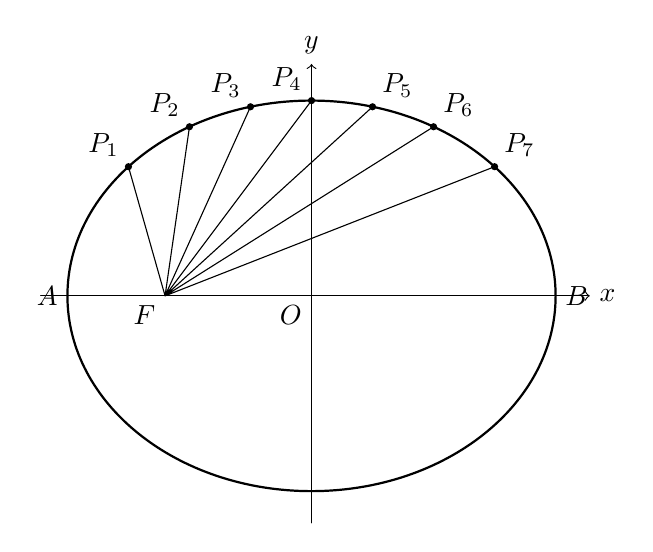
\begin{tikzpicture}[line cap=round,line join=round,x=0.62cm,y=0.62cm]
  \coordinate (P1) at (-3.75,2.646);
  \coordinate (P2) at (-2.50,3.464);
  \coordinate (P3) at (-1.25,3.873);
  \coordinate (P4) at (0,4);
  \coordinate (P5) at (1.25,3.873);
  \coordinate (P6) at (2.50,3.464);
  \coordinate (P7) at (3.75,2.646);
  \coordinate (F) at (-3,0);
  \draw[->] (-5.55,0)--(5.7,0) node[right] {$x$};
  \draw[->] (0,-4.65)--(0,4.75) node[above] {$y$};
  \draw[thick] (0,0) ellipse (5 and 4);
  \draw[thin] (F)--(P1) (F)--(P2) (F)--(P3) (F)--(P4)
              (F)--(P5) (F)--(P6) (F)--(P7);
  \foreach \i in {1,...,7} \fill (P\i) circle (1.3pt);
  \node[left] at (-5,0) {$A$};
  \node[right] at (5,0) {$B$};
  \node[below left] at (F) {$F$};
  \node[below left] at (0,0) {$O$};
  \node[above left] at (P1) {$P_1$};
  \node[above left] at (P2) {$P_2$};
  \node[above left] at (P3) {$P_3$};
  \node[above left] at (P4) {$P_4$};
  \node[above right] at (P5) {$P_5$};
  \node[above right] at (P6) {$P_6$};
  \node[above right] at (P7) {$P_7$};
\end{tikzpicture}
\end{center}
\nopagebreak[4]
\end{question}
\gkpart{三、解答题}

\begin{question}
\gkti{16}$m,n$ 是空间两条不同直线，$\alpha,\beta$ 是两个不同平面，下面有四个命题：

① $m\perp\alpha,\ n\parallel\beta,\ \alpha\parallel\beta\Rightarrow m\perp n$；

② $m\perp n,\ \alpha\parallel\beta,\ m\perp\alpha\Rightarrow n\parallel\beta$；

③ $m\perp n,\ \alpha\parallel\beta,\ m\parallel\alpha\Rightarrow n\perp\beta$；

④ $m\perp\alpha,\ m\parallel n,\ \alpha\parallel\beta\Rightarrow n\perp\beta$。

其中真命题的编号是\gkblank{}。（写出所有真命题的编号）

\end{question}
\begin{question}
\gkti{17}数列 $\{a_n\}$ 的前 $n$ 项和记为 $S_n$，$a_1=1$，$a_{n+1}=2S_n+1\ (n\geqslant1)$。

（1） 求 $\{a_n\}$ 的通项公式；

（2） 等差数列 $\{b_n\}$ 的各项为正，其前 $n$ 项和为 $T_n$，且 $T_3=15$，又 $a_1+b_1,a_2+b_2,a_3+b_3$ 成等比数列，求 $T_n$。

\end{question}
\begin{question}
\gkti{18}已知 $A\text{、}B\text{、}C$ 是 $\triangle ABC$ 三内角，向量 $\vec m=(-1,\sqrt3)$，$\vec n=(\cos A,\sin A)$，且 $\vec m\cdot\vec n=1$。

（1） 求角 $A$；

（2） 若 $\dfrac{1+\sin2B}{\cos^2B-\sin^2B}=-3$，求 $\tan C$。

\end{question}
\begin{question}
\gkti{19}某课程考核分理论和实验两部分进行，每部分考核成绩只记“合格”与“不合格”，两部分考核都“合格”则该课程考核“合格”。甲、乙、丙三人在理论考核中合格的概率分别为0.9、0.8、0.7；在实验考核中合格的概率分别为0.8、0.7、0.9。所有考核是否合格互相之间没有影响。

（1） 求甲、乙、丙三人在理论考核中至少有两人合格的概率；

（2） 求这三人该课程考核都合格的概率。（结果保留三位小数）

\Needspace{0.4\textheight}
\end{question}
\begin{question}
\gkti{20}如图，在长方体 $ABCD-A_1B_1C_1D_1$ 中，$E\text{、}P$ 分别是 $BC\text{、}A_1D_1$ 的中点，$M\text{、}N$ 分别是 $AE\text{、}CD_1$ 的中点，$AD=AA_1=a$，$AB=2a$。

（1） 求证：$MN\parallel$ 平面 $ADD_1A_1$；

（2） 求二面角 $P-AE-D$ 的大小。
\nopagebreak[4]
\begin{center}% Q20: cuboid with the marked midpoints and required segments.
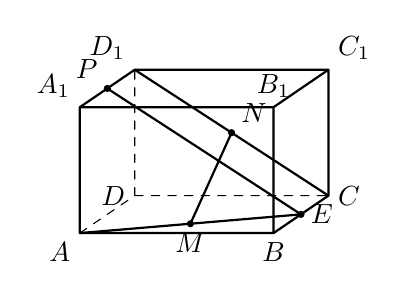
\begin{tikzpicture}[line cap=round,line join=round,x=0.82cm,y=0.82cm]
  \coordinate (A) at (0,0);
  \coordinate (B) at (3,0);
  \coordinate (C) at (3.85,0.58);
  \coordinate (D) at (0.85,0.58);
  \coordinate (Aone) at (0,1.95);
  \coordinate (Bone) at (3,1.95);
  \coordinate (Cone) at (3.85,2.53);
  \coordinate (Done) at (0.85,2.53);
  \coordinate (P) at (0.425,2.24);
  \coordinate (E) at (3.425,0.29);
  \coordinate (M) at (1.7125,0.145);
  \coordinate (N) at (2.35,1.555);

  % Rear edges are dashed; the front and right faces remain visible.
  \draw[dashed] (A)--(D) (D)--(C) (D)--(Done);
  \draw[thick] (A)--(B)--(C) (B)--(Bone)--(Cone)--(C)
               (A)--(Aone) (Aone)--(Bone) (Aone)--(Done)--(Cone) (A)--(B);
  \draw[thick] (A)--(E) (C)--(Done) (M)--(N) (P)--(E);
  \fill (P) circle (1.3pt) (E) circle (1.3pt) (M) circle (1.3pt) (N) circle (1.3pt);
  \node[below left] at (A) {$A$};
  \node[below] at (B) {$B$};
  \node[right] at (C) {$C$};
  \node[left] at (D) {$D$};
  \node[above left] at (Aone) {$A_1$};
  \node[above] at (Bone) {$B_1$};
  \node[above right] at (Cone) {$C_1$};
  \node[above left] at (Done) {$D_1$};
  \node[above left] at (P) {$P$};
  \node[right] at (E) {$E$};
  \node[below] at (M) {$M$};
  \node[above right] at (N) {$N$};
\end{tikzpicture}
\end{center}
\nopagebreak[4]
\end{question}
\begin{question}
\gkti{21}已知函数 $f(x)=x^3+3ax-1$，$g(x)=f'(x)-ax-5$，其中 $f'(x)$ 是 $f(x)$ 的导函数。

（1） 对满足 $-1\leqslant a\leqslant1$ 的一切 $a$ 值，都有 $g(x)<0$，求实数 $x$ 的取值范围；

（2） 设 $a=-m^2$，当实数 $m$ 在什么范围内变化时，函数 $y=f(x)$ 的图象与直线 $y=3$ 只有一个公共点。

\end{question}
\begin{question}
\gkti{22}已知两定点 $F_1(-\sqrt2,0),F_2(\sqrt2,0)$，满足条件 $\left|\overrightarrow{PF_2}\right|-\left|\overrightarrow{PF_1}\right|=2$ 的点 $P$ 的轨迹是曲线 $E$，直线 $y=kx-1$ 与曲线 $E$ 交于 $A,B$ 两点。

（1） 求 $k$ 的取值范围；

（2） 如果 $|\overrightarrow{AB}|=6\sqrt3$，且曲线 $E$ 上存在点 $C$，使 $\overrightarrow{OA}+\overrightarrow{OB}=m\overrightarrow{OC}$，求 $m$ 的值和 $\triangle ABC$ 的面积 $S$。

\end{question}